\documentclass[conference]{IEEEtran}
\usepackage[utf8]{inputenc}
\usepackage[german]{babel}

\usepackage{hyperref}

\usepackage{graphicx}
\graphicspath{figures/}

\makeatletter
\let\@copyrightspace\relax
\makeatother

\begin{document}

\title{MAC Authentication Bypass (MAB)\\ in Industrie 4.0}
\author{
	Umut-Vural Mitiler\\
	u.mitiler@stud.hs-wismar.de
	\and
	Fakultät für Ingenieurwissenschaften\\
	Hochschule Wismar\\
	Master IT-Sicherheit und Forensik\\
	Industrial Security\\
	Gruppe FFM-08
	\and
	David Schunke\\
	d.schunke@stud.hs-wismar.de
}

\maketitle

\thispagestyle{plain}
\pagestyle{plain}

%

\begin{abstract}
In dieser Abhandlung wird die port-based Network Access Control Methode MAC Authentication Bypass (MAB) sowie deren Bedeutung für die Industrie 4.0 diskutiert. Hierzu wird zunächst die grundsätzliche Motivation für Netzwerkzugangskontrolle dargestellt sowie eine Übersicht gegeben, was Industrie 4.0 bedeutet und definiert. Anschließend werden die technischen Grundlagen von MAB sowie den damit verbundenen Mechanismen und Standards - im speziellen Extensible Authentication Protocol (EAP) und IEEE802.1X - herausgearbeitet. Es wird zudem ein typisches Einsatzszenario als Fallback für RADIUS erläutert. Danach wird auf die Relevanz für die Industrie 4.0 sowie den bereits heute existierenden Einsatz in der Praxis eingegangen. Zum Schluss werden die Vorteile bzw. Nutzen sowie Nachteile und Gefahren diskutiert, und mögliche Gegenmaßnahmen analysiert. 
\end{abstract}

\vspace{1em}

\begin{IEEEkeywords}
MAC Authentication Bypass, MAB, EAP, Extensible Authentication Protocol, IEEE802.1X, dot1x, Network Access Control, NAC, Industrie 4.0, Schutzziele
\end{IEEEkeywords}

%

\vspace{1em}
\section{Motivation}
Die fortschreitende Vernetzung von IT Systemen bahnt sich ihren weg durch alle Bereiche unseres Lebens. Während ständige Vernetzung im Privaten- sowie Dienstleistungsumfeld heute alltäglich für uns sind, ist in der Industrie ein solcher Grad an Vernetzung noch nicht angekommen. So sind häufig im industriellen Umfeld noch Maschinen oder Systeme eingesetzt, welche aufgrund ihres Alters gar keine Vernetzung und Kommunikation erlauben, als auch existierende Vernetzungen lediglich für eine einfachste Form der Kommunikation, wie z.B. Systemüberwachung, eingesetzt.\\

Industrie 4.0 stellt die aktuellste und vierte Stufe der industriellen Revolution dar. Nachdem die erste industrielle Revolution durch die Mechanisierung von Arbeitsprozessen, die zweite industrielle Revolution durch den Einsatz technischer Hilfsmittel zur Massenproduktion, und die dritte industrielle Revolution erste digitale Hilfsmittel zur Automatisierung geprägt waren, werden in der vierten industriellen Revolution alle Komponenten digitalisiert, vollumfänglich vernetzt als auch mit Intelligenz versehen, sodass diese Komponenten teils vollautonom dezentrale Entscheidungen treffen und untereinander Kommunizieren können. Der Mensch interagiert nur noch eingeschränkt und teilweise über neuartige Schnittstellen (human-computer-interfaces, HCI) mit den Systemen, um diese z.B. bei Konflikten oder benötigten Entscheidungen anzuleiten. Solche Systeme werden Cyberphysische Systeme (CPS) genannt und bilden das Rückgrat der Industrie 4.0. \cite{botthof2015zukunft}\\

Mit Vernetzung und Kommunikation werden gleichzeitig solche Systeme allerdings auch stärker angreifbar und bedingen weitergehender Schutzmechanismen. Während in Office- oder User-Netzwerken Technologien und Protokolle zur Absicherung der Kommunikation bereits lange zum Standard gehören, sind die in der Industrie noch häufig eingesetzten Systeme und Protokolle auf eine Absicherung noch nicht ausgelegt. Gefahren bilden hierbei u.A.

\vspace{.5em}

\renewcommand{\labelenumi}{\alph{enumi})}
\begin{enumerate}
	\item Industriespionage durch Abfangen von Kommunikation oder eindringen in Systeme (Angriff auf die Vertraulichkeit)
	\item Manipulation von Kommunikation, z.B. Steuerbefehlen (Angriff auf die Integrität)
	\item Störung der (Echtzeit-)Kommunikation bis hin zu Denial-of-Service (DoS), sodass ein System komplett ausfällt (Angriff auf die Verfügbarkeit)
	\item Übernahme (Hijacking) von Systemen und missbräuchliche Verwendung oder Erpressung
\end{enumerate}

\vspace{.5em}

Die verschiedenen Gefahren stellen für die unterschiedlichen Zweige der Industrie auch unterschiedliche Schweregrade dar, sind jedoch in der Industrie 4.0 für alle Bereiche ein hochwichtiges Thema.\\

Ein zentraler Teil zur Absicherung der Schutzziele besteht darin, wer überhaupt Zugang zu einem Netzwerk bekommt, analog zur physischen Zugangsabsicherung zu einem Gebäude oder Areal. Im Alltag findet man heute zugangsoffene Wireless LAN nur noch selten. Meistens wird zur Authentifizierung ein Passwort oder auch Pre-shared Key (PSK) benötigt. Jeder mit diesem PSK kann sich zum Netzwerk verbinden. Im Bereich des wired LAN findet man allerdings auch heute noch oft völlig unbeschränkte Netzwerke, sodass jeder mit physischem Zugang sich verbinden könnte.\\

Die PSK Methode ist simpel, hat jedoch insbesondere zwei große Nachteile:
(a) es ist keine Unterscheidung der Teilnehmer möglich, d.h. jeder Teilnehmer hat auch die gleichen Möglichkeiten im Netzwerk, eine Limitierung Einzelner oder nach Gruppen ist nicht möglich, und
(b) je größer die Anzahl an Teilnehmern im Netzwerk, desto schwieriger wird es den PSK auszutauschen und zu erneuern, sodass dies mit der Zeit ein Sicherheitsrisiko darstellen kann.\\

Zur Lösung dieses Problems wurden bereits für Enterprise Netzwerke verschiedene Strategien und Technologien entwickelt, um eine Netzwerkzugangskontrolle (Network Access Acontrol, NAC) teilnehmergenau zu realisieren, und so eine genauere Authentifizierung sowie Autorisierung auf verschiedene Ressourcen in Form von Rechtevergabe zu ermöglichen.\\

Aufgrund des Alters vieler Systeme in der Industrie können diese Technologien allerdings nicht immer einfach übertragen werden, ohne Probleme in der Kompatibilität hervorzurufen, können gleichzeitig aber auch oft nicht einfach durch neue Systeme ausgetauscht werden. Dies betrifft u.A. Netzwerkdrucker, Sensoren, Kameras, älter Server, usw.\\

Aus diesem Grund werden für solche Systeme Fallback-Lösungen benötigt, sodass diese Systeme sich gegenüber der Netzwerkzugangskontrollinstanz authentifizieren und am Netzwerk teilnehmen können. Eine solche Fallback-Lösung stellt das \emph{MAC Authentication Bypass (MAB)} dar.
% todo italic stehen lassen? was alles italic / bold? %

%

\vspace{1em}
\section{Technische Grundlagen}
Zur Realisierung der Netzwerkzugangskontrolle wird eine zentrale Authentifizierungsstelle (Authentication Server) eingesetzt, sogenannte AAA-Server (Authentication, Authorization, Accounting). Jede Netzwerkkomponente (Authenticator), z.B. Router oder Switch, vergewissert sich bei ankommendem Netzwerkverkehr beim Authentication Server darüber, ob der Sender (Supplicant) authorisiert ist am Netzwerk teilzunehmen. Das \emph{Institute of Electrical and Electronics Engineers (IEEE)} hat hierfür den Standard \emph{IEEE802.1X} \cite{5409813} entwickelt, welcher wiederum die Nutzung des \emph{Extensible Authentication Protocol (EAP)} empfiehlt und somit quasi eine Verkapselung des EAP in einem Standard darstellt, weshalb im Folgenden zunächst das EAP erläutert wird.

\vspace{.5em}
\subsection{Extensible Authentication Protocol (EAP)}
Das EAP (RFC 3748 \cite{aboba2004extensible}) ist ein von der Internet Engineering Task Force (IETF) entwickeltes Framework zur Implementierung von Authentifizierung in Netzwerken. Es stellt Funktionen für verschiedene Authentifizierungsmethoden bereit, z.B. EAP-SIM, EAP-TTLS oder EAP-over-LAN (EAPOL). \cite{1561920} In \autoref{fig:eap} wird EAP als Abstraktionsebene dargestellt.\\

\begin{figure}[hbt]
	\centering
	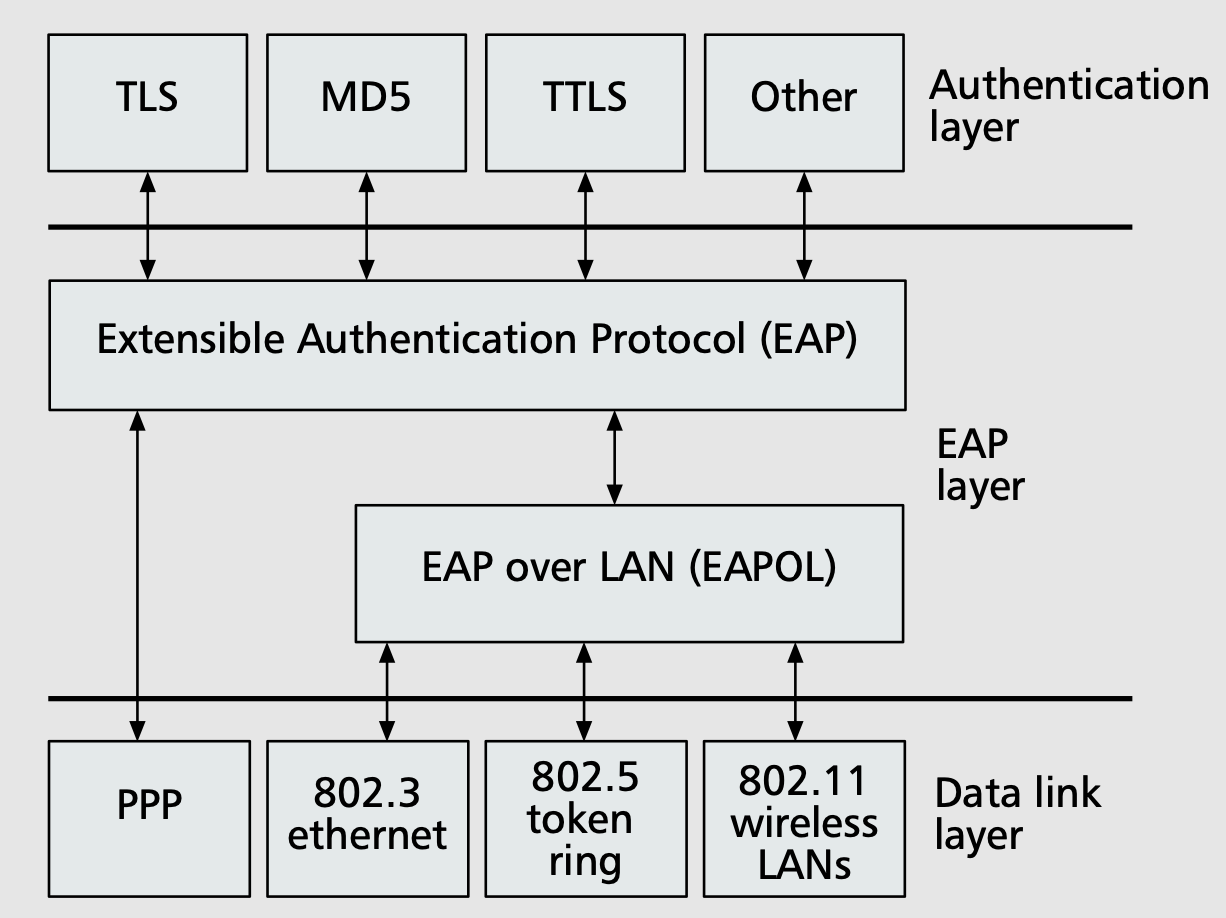
\includegraphics[width=9cm]{figures/EAP}
	\caption{EAP als Abstraktionsebene zur Authentifizierung (angelehnt an: \cite{1561920}).}
	\label{fig:eap}
\end{figure}

EAP wurde zur Unterstützung von Authentifizierung in Netzwerke geschaffen, ohne dass  bei einer neuen Authentifizierung die Infrastruktur angepasst werden müsste. Es erlaubt den Einsatz eines Authentication Servers (AAA) und implementiert die Prozesse zwischen Supplicant, Authenticator und Authentication Server. Hierbei können auch mehrere Methoden in Folge genutzt werden und erlaubt so heterogene Netzwerke. Nach Authentifizierungsanfrage (Authentication Request) vom Authenticator an den Supplicant sendet dieser eine Antwort, welche die konkrete Authentifizierung (Benutzer, Password, Zertifikat, etc.) enthält. Der Authenticator erfragt beim Authentication Server die Authentifizierung und schließt den Prozess mit einer Success- oder Failure-Response an den Supplicant ab.

\vspace{.5em}
\subsection{IEEE802.1X}
Der IEEE802.1X (kurz auch dot1x genannt) ist Teil der IEEE802.1 Gruppe von Standards \cite{5409813}. Es dient zur port-based Network Access Control (PNAC) und definiert Authentifizierungsmechanismen für LAN und WLAN. Hierzu setzt es auf das EAP over LAN (EAPOL) auf. In \autoref{fig:dot1x} wird die Funktionsweise und die einzelnen Parteien in dot1x dargestellt.\\

\begin{figure}[hbt]
	\centering
	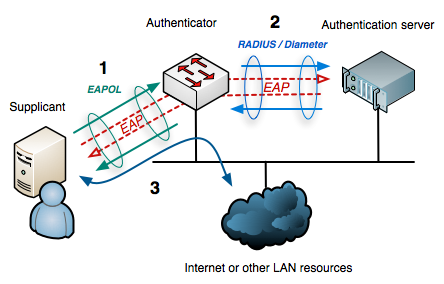
\includegraphics[width=9cm]{figures/dot1x}
	\caption{IEEE802.1X schrittweise in den einzelnen Parteien dargestellt (angelehnt an: \cite{eap}.}
	\label{fig:dot1x}
\end{figure}

Ports werden hierbei in zwei logische Einheiten unterteilt: (1) kontrollierte Ports und (2) unkontrollierte Ports. \cite{aboba2004extensible}\\
Kontrollierte Ports werden durch die dot1x PAE (Port Access Entity) gesteuert und lassen den Netzwerkverkehr für einen Supplicant entweder durch (authorized state) oder blocken diesen ab (unauthorized state).\\
Unkontrollierte Ports werden durch die dot1x PAE zur Übermittlung von EAPOL Paketen verwendet.

\vspace{.5em}
\subsection{RADIUS und Active Directory}
Oft als konkrete Implementierung eingesetzt werden RADIUS (Remote Authentication Dial-In User Service) oder Microsoft Active Directory. Diese bieten zentralisierte AAA-Server und sind dot1x konform, unterstützen also EAPOL. In \autoref{fig:radius} wird der Authentifizierungsprozess in Request / Response dargestellt.

\begin{figure}[hbt]
	\centering
	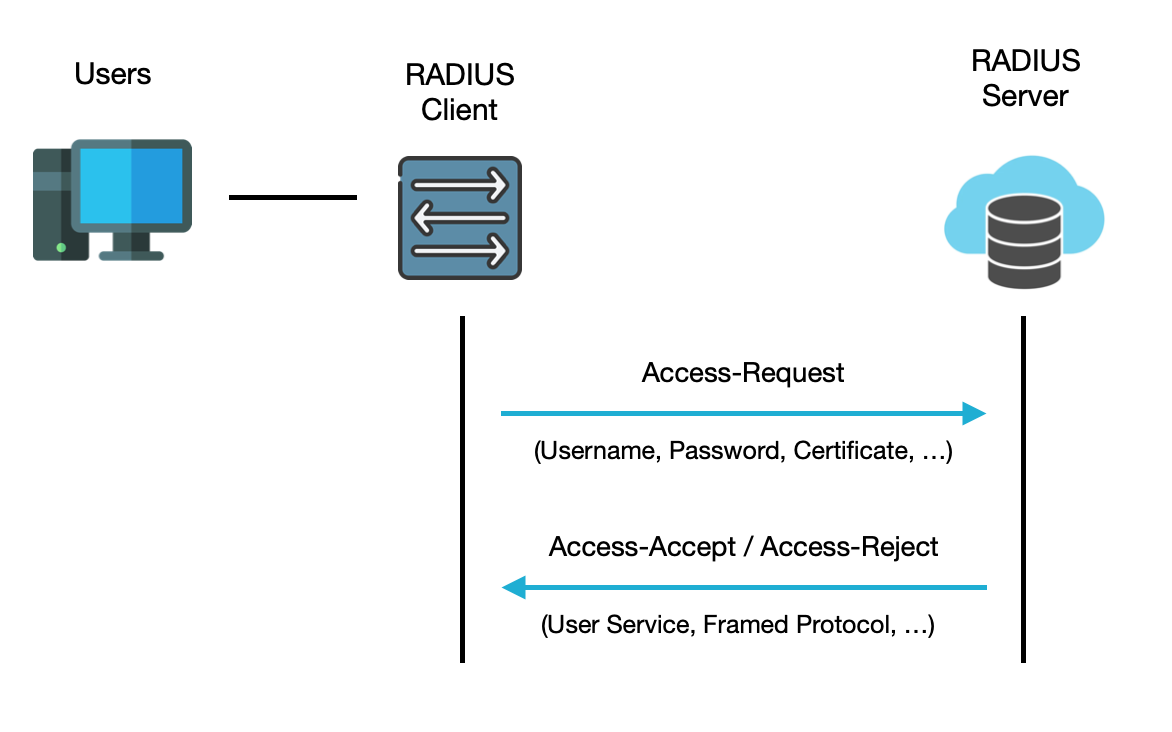
\includegraphics[width=9cm]{figures/radius}
	\caption{RADIUS Authentifizierung (angelehnt an: \cite{radius}).}
	\label{fig:radius}
\end{figure}

\vspace{.5em}
\subsection{Technische Umsetzung von MAB}
MAB wird meistens als Fallback für EAP / dot1x, also z.B. RADIUS, eingesetzt. Versucht ein Supplicant sich neu zu authentifizieren wird zunächst dessen Netzwerkverkehr geblockt. Der Authenticator versucht nun den Supplicant zu authentifizieren. Hierzu wird zunächst ein EAP-Request-Identity an den Supplicant gesendet, um die Authentifizierung zu initieren. Diesen Request versteht der Supplicant allerdings nicht, da er aufgrund Alters des System oder Niedrigkosten-optimierten Herrstellung EAP nicht implementiert. Diese EAP-Requests werden wiederholt, bis ein dot1x Timeout erfolgt, woraufhin die Authentifizierung abgebrochen wird. \cite{eap}\\

Anschließend beginnt die MAB Authentifizierung. Um die MAC-Adresse des Supplicant zu erlernen, wertet der Authenticator ein einzelnes Paket aus. Hierzu kann fast jedes beliebige Layer 2 oder 3 Paket genutzt werden. Der Authenticator sendet nun einen Access-Request an den Authentication Server. Dieser Request enthält in den Attributen \emph{Username} und \emph{Password} jeweils die MAC-Adresse des Supplicant. \cite{mab-deployment-guide} Lediglich das Format, in welchem die MAC-Adresse in den Attributen übertragen wird, unterscheidet sich. Zusätzlich findet sich in einigen Systemen noch das Attribute \emph{Calling-Station-ID} wieder, welches ebenfalls mit der MAC-Adresse befüllt und als sechs Gruppen mit jeweils zwei Hexadezimalstellen, in Großbuchstaben und mit Bindestrichen seperiert, übertragen wird. Welches Attribut konkret ausgewertet wird, hängt vom eingesetzten AAA-Server sowie dessen Konfiguration ab.\\

Der Authentication Server nimmt nun eine Bewertung vor und sendet entweder eine Accept oder Deny Response an den Authenticator zurück. Wichtige Voraussetzung hierzu ist, dass der Authentication Server die MAC-Adresse des Supplicant kennt, d.h. in einer Datenbank o.ä. zuvor eingepflegt wurde.\\

Der Authenticator erhält bei Erfolg ein Accept zurück und hat nun die MAC-Adresse des Supplicant erlernt. Der Supplicant ist nun auf diesem Port authentifiziert (authorised state) und kann Kommunizieren.

In \autoref{fig:mab-fallback} wird dieser Prozess noch einmal dargestellt.\\

\begin{figure}[hbt]
	\centering
	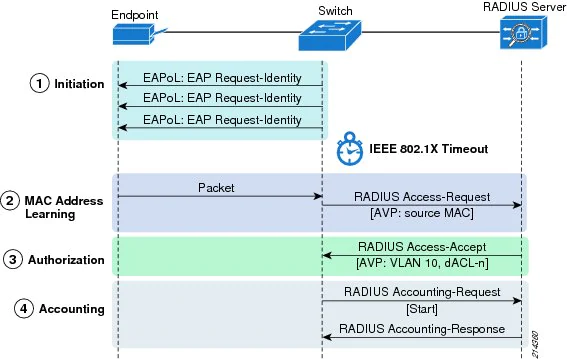
\includegraphics[width=9cm]{figures/mab-fallback}
	\caption{MAB als Fallback für RADIUS (Quelle: \cite{mab-deployment-guide})}
	\label{fig:mab-fallback}
\end{figure}

%

\vspace{1em}
\section{Praxiseinsatz}
In der Praxis wird MAB nicht nur als Fallback für RADIUS genutzt, sondern auch als zusätzliche Sicherheitsebene für \emph{NAC Network Authentication Control (NAC)}. Für Endgeräte die nicht über Layer 2 hinweg kommunizieren können, wie zum Beispiel IP-Phones, Kameras oder Drucker, die man dennoch nicht ungesichert im Netzwerk angeschlossen lassen möchte, bietet \emph{MAB} eine Möglichkeit diese Endgerät und weitere über verschiedene Mechanismen zu sichern.\\

\vspace{.5em}
\subsection{Heutiger Einsatz}
Heutzutage wird \emph{MAB} vor allem als Fallback genutzt, jedoch wie oben erwähnt, können durch das Provisionieren und Blockieren von MAC-Adressen auf verschiedenen Ebenen Policies erstellt werden um Endgeräte bereits auf Layer 2 Ebene im Netzwerk zu sperren. Zusätzlich dazu kann durch Architekturen gewährleistet werden, das diese MAC-Adressen durch ausgewählten User gepflegt werden, sodass die Datenbank in der sie provisioniert werden, nicht durch Dritte veränderbar ist. Dies verhindert zum einen Angriffe wie /emph{MAC-Spoofing}, sondern ermöglicht es auch mehrere hunderte oder tausende MAC-Adressen an einem zentralen Ort zu pflegen. Hierdurch kann eine Skalierbarkeit in die Breite ermöglicht werden, ohne die Architektur verändern zu müssen oder Endgeräte die nicht über Layer 2 hinweg kommunizieren können, aus dem Netzwerk auszusperren. Dies hat zusätzlich zu Folge, das Switches lokal nicht konfiguriert werden müssen, da die Policies und die Datenbank auf dem RADIUS-Server anliegen und die Switches lediglich mit diesem kommunizieren müssen.
Diese Konstellation bietet eine weitere Sicherheitsebene, da gewährleistet kann, dass der RADIUS-Server durch ausgewählte Administratoren gepflegt wird und die Switches bekannt sind. Dadurch kann eine Veränderung am Switch erkannt werden, falls diese vorliegt und ebenfalls durch Log-Einträge am RADIUS-Server erkannt werden, falls sich MAC-Adressen die am Switch liegen verändert haben. Allerdings birgt diese Konstellation ein Risiko, falls Switches durch Dritte ohne Überwachung ausgetauscht werden können, dies öffnet wiederrum den Angriffswinkel das MAC-Spoofings.\\

\begin{figure}[hbt]
	\centering
	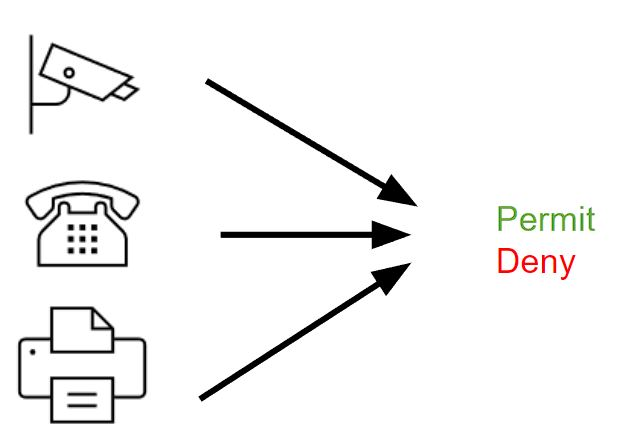
\includegraphics[width=9cm]{figures/MAB_heutiger_Einsatz}
	\caption{Heutiger Einsatz für MAB}
	\label{fig:mab-today}
\end{figure}

\vspace{.5em}
\subsection{Relevanz in Industrie 4.0}
Die Relevanz von \emph{MAB} in der Industrie 4.0 bezieht sich nicht auf die Verfügbarkeit in der Zukunft, sondern darauf wie mit Endgeräten, wie bereits oben erwähnt, die nicht über Layer 2 hinweg kommunizieren können. Hier werden Punkte wie  eine hoch flexible Verknüpfung der Datenebene \cite{hirsch2014wandel} erwähnt. Hier bietet die Möglichkeit von MAB nicht nur als Fallback für RADIUS, sondern insbesondere als Sicherheitsebene zu dienen, eine großen Vorteil die oben erwähnte flexible Verknüpfung zu schaffen. Ein weiterer Punkte der relevant ist für die Industrie wäre die Beherrschung komplexer Systeme \cite{botthof2015zukunft}, da zusätzlich zu den in den letzten Jahren angestiegenen Zahlen der IoT-Geräte, auch ''Leichen'' die durch das ausbauen von Netzen mitgetragen werden, weiterhin sicher angebunden werden müssen. Hierbei kann die weiter oben erwähnte Maßnahme von Pflegen und Provisionieren von MAC-Adressen sehr praktikabel sein, da die Erweiterung von Netzwerken und Technologien keine Kompromitierung darstellen sollte, sonderen diese nur erweitern und im besten Falle auch verbessern soll. Im weiteren Sinne kann die Skalierbarkeit die MAB bietet auch als weiterer Vorteil für eine flächendeckende Breitbandinfrastruktur \cite{botthof2015zukunft} dargestellt werden. In  Sendlers ''Industrie 4.0 grenzenlos'' wird auch die verengte Sicht auf die Produktion als Negativbeispiel genannt\cite{sendler2016industrie}, da historisch diese bei industriellen Revolutionen am meisten Aufwand erzeugt und immer wieder optimiert werden musste.\\

Weiterhin nennt er auch, dass in der Industrie 4.0 auf Dienstleister und alle weiteren Aspekte einer Wertschöpfungskette geachtet werden muss falls diese Revolution erfolgreich sein soll. Wie weiter oben erwähnt, gehören hier auch die Altlasten hinzu die, im wachsenden Netzwerk von IoT-Geräten, immer weniger an Bedeutung innehaben, jedoch weiter betrachten werden müssen, sei es als Glied der Wertschöpfungskette oder als Dienstleister für andere Produzenten. Auf diesen Punkt spielt jedoch die Analyse Industrie 4.0–Vorgehensmodell für die Einführung ein. Hier wird untersucht ob und wie die bereits bestehenden Produkt- und Prozessebenen angepasst werden müssen und inwiefern diese die Industrie 4.0 wiederspiegeln \cite{lucia2016industrie}. Diese Analyse, entgegen der Punkte die oben genannt wurden, spiegeln eine akkuratere Anpassung einer Wertschöpfungskette an die Industrie 4.0 und können durch konkrete Ist- und Sollanalysen verglichen und an die Entwicklung eines Unternehmens oder eines Prozesses angepasst werden.\\

%

\vspace{1em}
\section{Ergebnis}
Zusammenfassend lassen sich die Möglichkeiten und sicherheitstechnischen Elemente von MAB in verschiedenen Aspekten aufzeigen. Einerseits, und dies ist der offensichtlichste Faktor, Endgeräte, die nicht über Layer 2 hinweg kommunizieren können, in eine heterogene Netzwerklandschaft miteinbeziehen, ohne größere Sicherheitsrisiken einzugehen. Dies ist vor allem durch zentrales Provisionieren, Pflegen von Datenbanken und dem konkreten Ausschließen von unbekannten MAC-Adressen möglich. Dies verursacht zwar einen gewissen Aufwand auf Seiten von Netzwerkadministratoren und Haltern von Endgeräten, da diese zuerst aufgenommen und gepflegt werden müssen, jedoch kann durch den Aufbau von Prozessen und Policies durch die diese Endgeräte durchlaufen, gewährleistet werden, dass neue Endgeräte ebenfalls schneller und sicherer ans Netz gebracht werden können. Durch Architekturen und RADIUS-Server wie die Cisco ISE, lässt sich dies ebenfalls, wie bereits erwähnt, in einer flexiblen Verknüpfung für breite Netzwerklandschaften erfüllen. Abgesehen davon MAB als Sicherheitsebene zu nutzen, lässt sich die Funktion auch als Fallbackebene für Endgeräte nutzen, die sich bereits im Netzwerk befinden. Dies kann nützlich sein, falls bei EAP-basierten Verbindungen Fehler auftreten oder in Netzwerken mehrere Ebenen und Möglichkeiten von Verbindungsmöglichkeiten aufgesetzt werden. Hierbei kann MAB als Fallbackebene für jegliche Endgeräte genutzt werden, da diese ebenfalls eine MAC-Adresse im Netzwerk innehaben und diese gepflegt und in Datenbanken provisioniert werden kann.\\

%

An diesen Punkt lassen sich auch die Vor- und Nachteile von MAB aufzählen. Wie eben erwähnt lääst sich die Sicherheitsebene relativ einfach durch Abfragen von MAC-Adressen realisieren. Im Beispiel weiter oben wurde die Archtitektur von Cisco erwähnt auf der diese Authentifizierunsmethode basiert. Hierbei werden Endgeräte nach ihren MAC-Adressen sortiert und Policies auf Basis dieser Gruppen erstellt. Am Ende jeder Policy steht ein Deny-All, dies hat zur Folge das jegliche Endgeräte die zu keiner dieser Gruppen passen, von dem RADIUS-Server nicht authentifiziert werden. Dabei ist zu erwähnen, dass keine zertifikatsbasierte Authentifierung nicht notwendig ist. Somit ist die Pflege von Zertifikaten, obgleich dies nun eine intern- oder extern-basierte Zertifikatsinfrastruktur ist, von vornherein ausgeschlossen. Zusätzlich dazu benötigt der Switch nur ein einzelnes Paket, um die MAC-Adresse des Endgeräts zu erfahren, dass versucht sich zu authentifizieren. Damit ist die Netzwerklast geringer als durch zertifikats- oder Username-Passwort-basierten Authentifizierungsmethoden. Dies basiert alles darauf, das nicht über Layer 2 hinweg kommuniziert werden muss, dadurch wird erst keine TCP-IP Verbindung aufgebaut und es kann rein auf der Data-Link-Layer kommuniziert werden.\\

\begin{figure}[hbt]
	\centering
	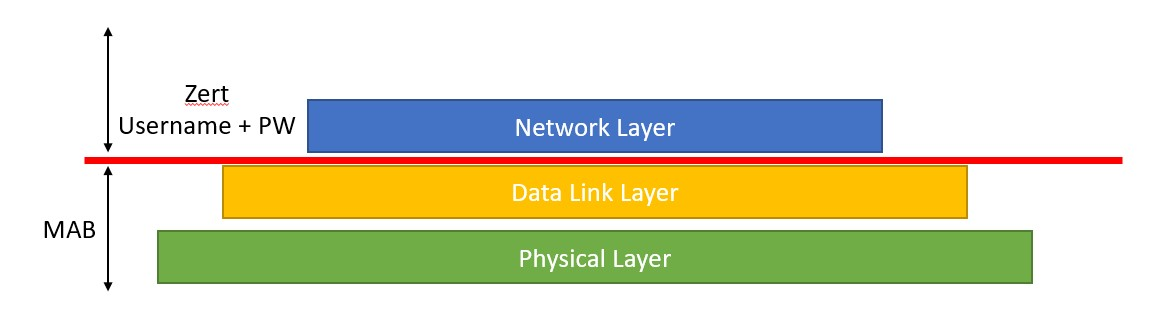
\includegraphics[width=9cm]{figures/MAB_Layer_2.jpg}
	\caption{Grenze von endgerätebasierter und userbasierter Authentifizerung}
	\label{fig:mab}
\end{figure}

Jedoch ist hier auch zu erwähnen, das gewisse Nachteile bei Nutzung von MAB entstehen. Zunächst muss die Pflege der Datenbanken erwähnt werden, da dies bei relativ kleinen Unternehmen übersichtlich erscheinen kann, jedoch kann wird diese ja nach Größe des Unternehmens sehr schnell unübersichtlich. Anbindung und Pflege von mehreren tausend Endgeräten, vor allem wenn diese erst neu dokumentiert werden müssen, kann schnell zu einem Mehraufwand werden, die sich aus Sicht von Kosten-Leistungs-Analysen nicht zu lohnen scheinen mag. Hier muss Zweck gegen Risiko ausgewogen werden, und ob diese Geräte überhaupt noch am Netz angebunden bleiben sollen.\\

Weiterhin, wie bereits oben erwähnt ist keine personenbezogene Authentifizierung möglich. Da weder zertifikats- noch Username-Passwort-basierte Authentifizierung auf Layer 2 möglich ist, kann nur das Endgerät authentifiziert werden und der Nutzer des Endgeräts nicht. Dies erschwert die Einbindung von Identity und Access Management in diese Form von Authentifizierung. Zusätzlich dazu müssen die Switches an denen MAB durchgeführt werden soll, konfiguriert werden, sodass sie mit dem RADIUS-Server kommunizieren können und durch diesen auch authentifiziert werden können. Dies kann je nach Anzahl der zu konfigurierenden Switches einen erheblichen Mehraufwand erzeugen, vor allem wenn diese händisch aufgespielt werden sollen.\\

\begin{figure}[hbt]
	\centering
	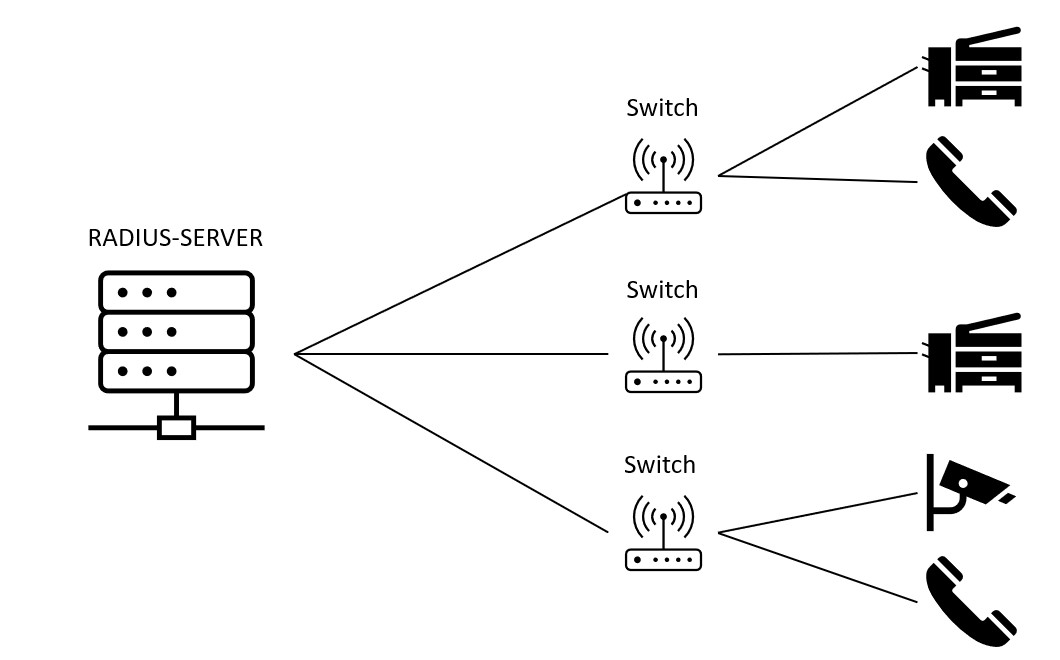
\includegraphics[width=9cm]{figures/Server_Switch.jpg}
	\caption{Architektur Skizze einer MAB-Konfiguration}
	\label{fig:mab_configuration}
\end{figure}

Letztlich ist noch der relativ einfache Angriffswinkel des Spoofings aufzunehmen, denn falls die Switches offenliegen und durch Dritte austauschbar sind, kann dies zum Vorteil eines Angreifers ausgenutzt werden, um Endgeräte im Netz zu authentifizieren und so eine Tür zu öffnen. Dies kann durch konkretes Absichern der Switches durch Schutzschränke erreicht werden oder durch Anbringen der Switches an Orten an die Angreifer ohne Weiteres nicht herankommen, wie zum Beispiel an hohen Decken. Hierbei können Angreifer entweder den Switch selbst austauschen, um diesen als Angriffsvektor zu nutzen oder an einem bestehenden Switch ein Endgerät, bei dem die MAC-Adresse bekannt ist, vortäuschen um so Informationen über das Netzwerk zu gewinnen.\\

\begin{figure}[hbt]
	\centering
	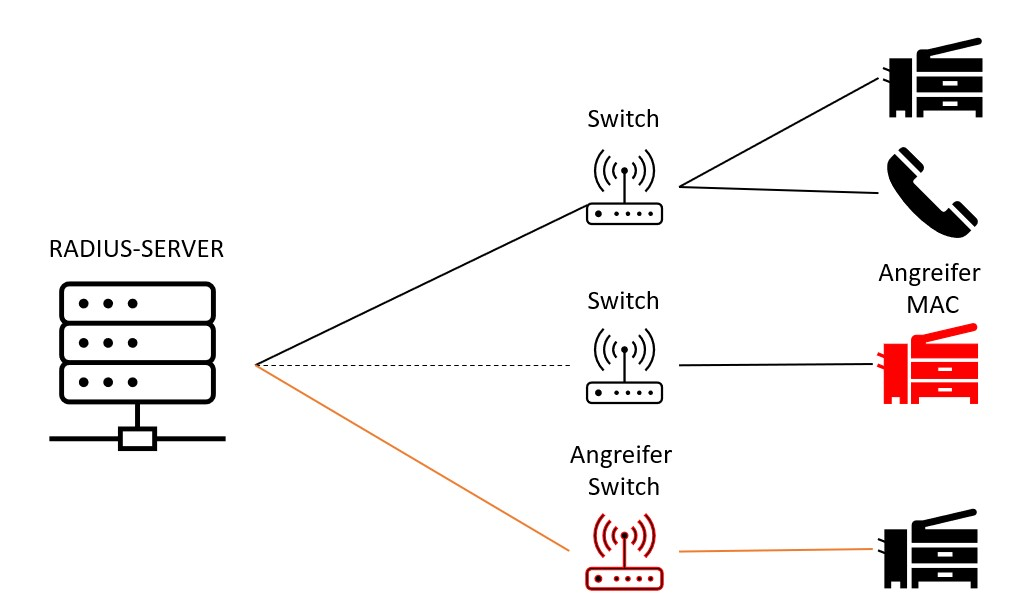
\includegraphics[width=9cm]{figures/Angriffsszenario_Spoofing.jpg}
	\caption{Angriffsszenario MAC-Spoofing}
	\label{fig:mac_spoofing}
\end{figure}

Zuletzt sollte noch darauf eingegangen werden, wie zukunftsträchtig MAB ist und inwiefern es möglich ist, diese Architektur in der Industrie 4.0 zu nutzen oder ob sie dafür nicht geeignet ist.\\

Wie weiter oben bereits erwähnt werden in heutigen Analysen in Bezug auf die Industrie 4.0 hauptsächlich neue Infrastrukturen, IoT-Geräte oder komplexe Systeme betrachtet. Jedoch wird selten in diesen Analysen auf die Altlasten und ''Leichen'' in Architekturen und Netzwerken eingegangen. In Ist- und Sollanalysen muss jedoch zwingend auf diese eingegangen werden, damit im Ausbau und in der Weiterentwicklung durch diese Altlasten keine Komplikationen auftreten die man im Nachhinein auflösen muss. Von daher hat MAB aus diesem Blickwinkel eine gewisse Daseinsberechtigung. Jedoch müssen die Vorteile und die Nachteile abgewogen werden, um nicht nur Die Sicherheitsvorteile, sondern auch den Aufwand aufzuzeigen.\\

In zukunftsorientierten Architekturen und Netzwerken die sich immer weiter in Richtung der Industrie 4.0 bewegen, ist es natürlich nicht abdingbar auch die Altlasten die sich im System bewegen weiterhin sicher anzubinden. Hierbei bietet MAB eine gute und relativ einfach aufzusetzende Alternative. Jedoch muss hierbei, je nach Größe der Netzwerke und der anzubindenden Endgeräte kann dies jedoch einen Mehraufwand erzeugen, bei dem dieser Aufwand gegenüber von neu anzuschaffenden Gerät aufgewogen werden muss. In der Regel ist es sinnvoller durch MAB diese Endgeräte anzubinden und per RADIUS-Server zu authentifizieren, da dies ebenfalls eine Möglichkeit bietet, einen Überblick aller vorhandenen Endgeräte zu schaffen und gleichzeitig ungenutzte Geräte auszuschließen oder gleich zu ersetzen. In der Regel heißt dies auch, dass hierdurch ein Fallback geschaffen werden kann, um Geräte bei DNS-, PKI oder AD-Problemen durch MAB im Netz zu halten, um zum Beispiel Produktivität aufrechtzuerhalten oder Endgeräte wie Kameras am laufen zu halten ohne diese weiter ins Netz einbinden zu müssen.\\

Als Fazit lässt sich also sagen, dass MAB eine gute Möglichkeit bietet, ein Sicherheitsniveau zu schaffen und gleichzeitig ein Fallback einzurichten. Hierbei muss jedoch der Mehraufwand aufgebracht werden, um dieses Niveau zu erreichen, die weitere Pflege ist jedoch im Vergleich etwas einfacher aufrechtzuerhalten.

%

\vspace{1em}
\bibliographystyle{IEEEtran}
\bibliography{references}

\end{document}